\documentclass[10pt,twocolumn,letterpaper]{article}

\usepackage{cvpr}
% \usepackage{times}
\usepackage{epsfig}
\usepackage{graphicx}
\usepackage{amsmath}
\usepackage{amssymb}
\usepackage{booktabs}
\usepackage{multirow}
\usepackage{microtype}
\usepackage{xcolor}
\usepackage{tikz}
\usetikzlibrary{arrows.meta, positioning, fit, backgrounds, calc}

\usepackage[breaklinks=true,bookmarks=false]{hyperref}

\cvprfinalcopy % *** Uncomment this line for the final submission

\def\cvprPaperID{****} % *** Enter the CVPR Paper ID here
\def\httilde{\mbox{\tt\raisebox{-.5ex}{\symbol{126}}}}

% ── Color palette (same as proposal) ──────────────────────
\definecolor{cblue}{RGB}{214,234,248}
\definecolor{cred}{RGB}{250,219,216}
\definecolor{cgreen}{RGB}{213,245,227}
\definecolor{cgray}{RGB}{240,240,240}

% ============================================================

\title{PAPIT: Prompt-Aware Pruning for Image Tokens\\
       in Efficient Multimodal Inference}

\author{%
  Chao Hsuan Ho \quad Heng Jui Hsu \quad Kerstin Sun \\
  Department of Computer Science, Rice University \\
  {\small\texttt{\{ch218, hh83, ks256\}@rice.edu}}
}

\setcounter{page}{1}
\begin{document}
\maketitle

% ============================================================
\begin{abstract}
Multimodal Large Language Models (MLLMs) such as LLaVA encode images
as hundreds of visual patch tokens, most of which are irrelevant to a
given user query. A natural hypothesis is that CLIP-derived
cross-modal saliency, which is already query-conditioned and requires
no training, can identify the relevant tokens. We test this
hypothesis with \textbf{PAPIT} (\textbf{P}rompt-\textbf{A}ware
\textbf{P}runing for \textbf{I}mage \textbf{T}okens), a training-free
pipeline that scores visual patches against the user's prompt using
GradCAM saliency on LLaVA's own vision tower and retains only the
top-$k$ most relevant tokens before LLaVA inference. Efficiency
experiments confirm a 41--90\% reduction in attention FLOPs with
negligible scoring overhead. However, on three VQA benchmarks (700
samples each), PAPIT only matches a query-agnostic random baseline:
GQA 69.7\% vs.\ 70.1\%, VQA~v2 74.8\% vs.\ 75.8\%, TextVQA 42.9\% vs.\
42.0\% at $k{=}75\%$. To explain this, we directly measure the
alignment between PAPIT's GradCAM scores and LLaVA's internal
attention over the 576 image tokens on 100 samples per benchmark,
and find on all three datasets a per-image Spearman $\rho \approx 0$
with top-$10\%$ Jaccard \emph{below} the uniform-random baseline. Our main contribution is therefore a
quantitative \emph{negative result}: CLIP-aligned saliency carries
essentially no information about which patches the LLM relies on,
ruling out an entire family of training-free prompt-aware pruning
approaches. As a positive control, we test an LLM-internal-attention
oracle on the same pipeline and find that mid-layer attention
($L\!\approx\!16$ in LLaVA-1.5-7B) does beat random ($+0.08$ at
$k\!=\!25\%$, matching unpruned at $k\!=\!50\%$ on GQA-100), showing
that prompt-aware pruning is achievable provided the signal is read
from inside the LLM rather than from the CLIP-aligned vision side.
\end{abstract}

% ============================================================
\section{Introduction}

LLaVA-1.5~\cite{liu2024llava15} processes a 336$\times$336 image as a
$24\!\times\!24 = 576$ patch token grid via a CLIP ViT-L/14 vision
encoder~\cite{dosovitskiy2021vit,radford2021clip}. Each token
participates in every self-attention
layer~\cite{vaswani2017attention} of the language model, making
inference cost quadratic in the number of visual tokens. For a typical
VQA query, fewer than half of these tokens are semantically relevant.

A natural intuition is that the user's prompt should be enough to
identify which tokens to keep, \emph{without} any training, since CLIP
and its derivatives already provide a query-conditioned cross-modal
embedding space. We ask: \emph{can a training-free saliency signal,
read from LLaVA's own CLIP-initialized vision tower, predict which
patches the LLaVA LLM actually relies on, well enough to beat a
query-agnostic random baseline?}

We instantiate this as \textbf{PAPIT}, a training-free pipeline that
scores patches by GradCAM saliency on LLaVA's vision tower against
the prompt's CLIP text embedding, retains the top-$k$ patches plus a
global anchor, and feeds the pruned set through LLaVA's MLP projector
and LLM. Across three VQA benchmarks, PAPIT \emph{ties} random
pruning rather than beating it (Sec.~\ref{sec:experiments}), even
though Figure~\ref{fig:qualitative} shows interpretably localised
selection on individual examples. An alignment diagnostic
(Sec.~\ref{sec:diagnostic}) on 100 samples from each of the three
benchmarks explains why: per-image Spearman $\rho \approx 0$ between
PAPIT's GradCAM scores and LLaVA's LLM attention over the 576 image
tokens, and the top-$10\%$ Jaccard falls slightly \emph{below} the
uniform-random reference on every dataset.

\paragraph{Contributions.}
(i) A clean training-free token-pruning pipeline for LLaVA-1.5 with
41--90\% attention-FLOPs reduction and $\le$2.3-point accuracy loss
vs.\ unpruned on GQA and VQA~v2 at $k{=}75\%$. (ii) A quantitative
\emph{negative result}: CLIP-derived patch saliency is statistically
uncorrelated with LLaVA's LLM attention, which rules out an entire
family of training-free prompt-aware methods and motivates
LLM-internal scoring (FastV-style attention, or trained predictors
over LLaVA hidden states) for any future
prompt-conditioned approach.

% ============================================================
\section{Related Work}

Token pruning for Vision Transformers has been studied for image
classification~\cite{rao2021dynamicvit, meng2022adavit}, where a learned
predictor module decides which tokens to drop.
In the multimodal setting, FastV~\cite{chen2024fastv} prunes visual tokens
based on attention scores inside the LLM, requiring a forward pass before
pruning.
A complementary line of work shows that dense patch-level signals can be
extracted directly from CLIP without supervision, e.g.\ MaskCLIP~\cite{zhou2022maskclip},
motivating the use of CLIP-derived saliency for query-conditioned scoring.
PAPIT differs in that pruning happens \emph{before} the LLM sees the image,
using a lightweight cross-modal scoring step ($\approx$85\,ms, dominated by
the CLIP text-encoder forward pass) that is entirely query-conditioned and
requires no training.

% ============================================================
\section{Methodology}
\label{sec:method}

\subsection{Pipeline Overview}

Figure~\ref{fig:pipeline} shows the three-stage pipeline.
PAPIT reuses LLaVA-1.5's frozen vision tower, which is itself a CLIP
ViT-L/14, so no second image encoder is loaded; only the matching CLIP
text encoder is added on top to obtain a text embedding for cross-modal
scoring.
The image is encoded by the (shared) ViT and the prompt by the CLIP text
encoder; GradCAM scoring then selects the top-$k$ most relevant patches;
the pruned tokens are projected by LLaVA's MLP projector and fed to the
LLM to generate an answer.

% ── TikZ pipeline ─────────────────────────────────────────
\begin{figure}[htbp]
\centering
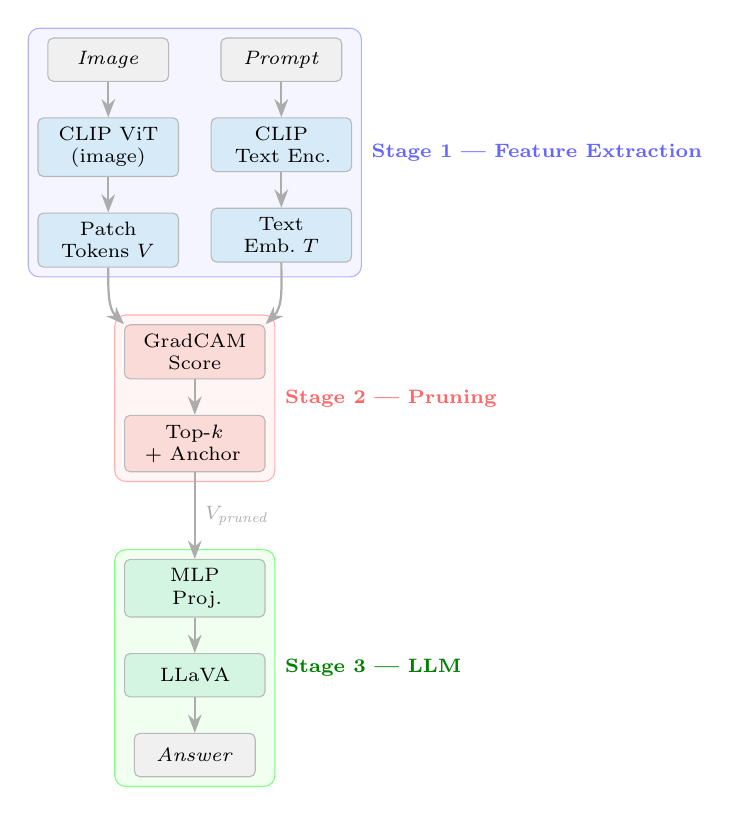
\begin{tikzpicture}[
  node distance = 0.45cm and 0.65cm,
  box/.style    = {rectangle, rounded corners=2pt, draw=gray!55,
                   fill=#1, text width=1.55cm, align=center,
                   minimum height=0.55cm, font=\scriptsize},
  iobox/.style  = {rectangle, rounded corners=2pt, draw=gray!55,
                   fill=cgray, text width=1.30cm, align=center,
                   minimum height=0.55cm, font=\scriptsize\itshape},
  arr/.style    = {-Stealth, thick, gray!65},
  sublbl/.style = {font=\tiny\itshape},
]
% Row 1: inputs
\node[iobox]                       (img)  {Image};
\node[iobox, right=0.65cm of img]  (txt)  {Prompt};
% Row 2: encoders
\node[box=cblue, below=0.45cm of img]  (vit)  {CLIP ViT\\(image)};
\node[box=cblue, below=0.45cm of txt]  (clip) {CLIP\\Text Enc.};
% Row 3: embeddings
\node[box=cblue, below=0.45cm of vit]  (vtok) {Patch\\Tokens $V$};
\node[box=cblue, below=0.45cm of clip] (temb) {Text Emb.\ $T$};
% Row 4–5: pruning (centred between the two columns)
\node[box=cred, below=1.1cm of $(vtok)!0.5!(temb)$] (score){GradCAM\\Score};
\node[box=cred, below=0.45cm of score]               (topk) {Top-$k$\\+ Anchor};
% Row 6–8: LLM
\node[box=cgreen, below=1.1cm of topk]  (mlp)  {MLP\\Proj.};
\node[box=cgreen, below=0.45cm of mlp]   (llava){LLaVA};
\node[iobox,      below=0.45cm of llava] (out)  {Answer};
% Arrows
\draw[arr] (img)  -- (vit);
\draw[arr] (vit)  -- (vtok);
\draw[arr] (txt)  -- (clip);
\draw[arr] (clip) -- (temb);
\draw[arr] (vtok.south) to[out=270,in=135] (score.north west);
\draw[arr] (temb.south) to[out=270,in=45]  (score.north east);
\draw[arr] (score) -- (topk);
\draw[arr] (topk)  -- node[right, font=\scriptsize\itshape]{$V_{\text{pruned}}$} (mlp);
\draw[arr] (mlp)   -- (llava);
\draw[arr] (llava) -- (out);
% Background stage boxes
\begin{pgfonlayer}{background}
  \node[draw=blue!30, fill=blue!4, rounded corners=4pt,
        fit=(img)(vit)(vtok)(txt)(clip)(temb),
        label={[font=\scriptsize\bfseries, blue!60]right:Stage 1 — Feature Extraction}] {};
  \node[draw=red!30, fill=red!4, rounded corners=4pt,
        fit=(score)(topk),
        label={[font=\scriptsize\bfseries, red!60]right:Stage 2 — Pruning}] {};
  \node[draw=green!50, fill=green!6, rounded corners=4pt,
        fit=(mlp)(llava)(out),
        label={[font=\scriptsize\bfseries, green!50!black]right:Stage 3 — LLM}] {};
\end{pgfonlayer}
\end{tikzpicture}
\caption{PAPIT pipeline. Pruning happens between the ViT and the LLaVA
         MLP projector, requiring no modification to the LLM weights.}
\label{fig:pipeline}
\end{figure}

\subsection{Cross-Modal Scoring: GradCAM Saliency}

Because CLIP's contrastive objective aligns only the CLS token with text,
naïve patch--text cosine similarity is unstable across retention ratios
and collapses at $k{=}50\%$ (Table~\ref{tab:ablation}); GradCAM saliency
on the vision tower provides a more reliable patch-level signal,
as confirmed by the ablation in Section~\ref{sec:experiments}.

\paragraph{GradCAM scoring.}
Let $H^{(L-1)} = \{h_1,\ldots,h_n\}$ denote patch activations at the
penultimate ViT encoder layer, and $\text{sim}$ the cosine similarity
between the projected CLS image embedding and the text embedding $T$.
We attribute $\text{sim}$ to each patch via GradCAM~\cite{selvaraju2017gradcam}:
\begin{equation}
  s^{\text{gc}}_i = \operatorname{ReLU}\!\left(
        \sum_{d}\, \frac{\partial\,\text{sim}}{\partial\, h_{id}}\cdot h_{id}
        \right).
  \label{eq:gradcam}
\end{equation}
Backpropagating through the final attention layer captures each patch's
\emph{causal} contribution to the global text-image alignment.
The top-$k$ patches are retained:
$V_{\text{pruned}} = \{h_i \mid s^{\text{gc}}_i \in \text{TopK}(\{s^{\text{gc}}_j\}_{j=1}^{n},\, k)\}$.

\subsection{Spatial Anchoring}

After top-$k$ selection, the pruned tokens preserve their original 2-D
grid indices as position IDs before being passed to the MLP projector.
One \emph{anchor token} (mean of all dropped tokens) is appended to
provide global context, giving a final sequence of length $k+1$.

\subsection{Efficiency Reduction}

Self-attention cost scales quadratically with sequence length.
Let $L_{\text{text}}$ be the number of text tokens (typically $\approx$50).
Relative FLOPs compared to unpruned inference is:
\begin{equation}
  \text{FLOPs}_{\text{rel}} =
  \frac{(k + L_{\text{text}})^2}{(n + L_{\text{text}})^2}.
  \label{eq:flops}
\end{equation}
For LLaVA-1.5 with $n=576$: retaining $k=25\%$ ($144$ tokens) yields
$\text{FLOPs}_{\text{rel}} \approx 0.10$, a $\sim$10$\times$ reduction.

\subsection{Implementation}

PAPIT operates at the token level between the ViT encoder and the
LLaVA MLP projector, requiring no modification to LLM weights.
The image branch reuses LLaVA-1.5's own vision tower (a frozen CLIP
ViT-L/14); the text branch loads the matching \texttt{clip-vit-large-patch14}
text encoder via HuggingFace Transformers, so the only extra parameters
introduced by PAPIT are CLIP's text encoder weights.

% ============================================================
\section{Qualitative Results}

\begin{figure*}[t]
  \centering
  
\includegraphics[width=\textwidth]{fig_qualitative_GQA.pdf}
  \caption{\textbf{Prompt-aware patch selection} on two GQA examples ($k{=}50\%$).
           \textit{Top:} original image and GradCAM saliency (warm = high score).
           \textit{Bottom:} PAPIT-selected vs.\ randomly selected patches (black = dropped).
           PAPIT preserves semantically relevant regions; random selection scatters uniformly.}
  \label{fig:qualitative}
\end{figure*}

Figure~\ref{fig:qualitative} illustrates prompt-aware patch selection on two GQA examples.
In the first example, GradCAM highlights the player region in response to a jersey-colour query,
and PAPIT's retained patches are visibly more concentrated on the subject than random selection.
In the second example, the strong colour contrast between the orange umbrella and blue sky
produces a clear saliency map: GradCAM assigns high scores to the umbrella boundary, and
PAPIT's selection concentrates on the umbrella area while random selection scatters across
the irrelevant sky, demonstrating a case where prompt-aware scoring provides an interpretable
spatial advantage.

% ============================================================
\section{Quantitative Results}

We conducted an efficiency benchmark using a BLIP~\cite{li2022blip} VQA proxy model
(Table~\ref{tab:efficiency}) and a full LLaVA-1.5 accuracy evaluation
on GQA~\cite{hudson2019gqa}, VQA~v2~\cite{goyal2017vqav2}, and TextVQA~\cite{singh2019textvqa}
(Table~\ref{tab:accuracy}).
The proxy model uses a $7\!\times\!7 = 49$ patch grid;
full LLaVA experiments use $n=576$.

\begin{table}[htbp]
\centering
\small
\caption{Efficiency benchmark results (BLIP proxy model, single A6000 GPU,
         averaged over 3 runs per setting).
         Prune latency includes CLIP scoring + top-$k$ selection.
         E2E latency includes pruning and the BLIP forward pass.}
\label{tab:efficiency}
\begin{tabular}{@{}lccccc@{}}
\toprule
$k$ & Tokens & Keep & FLOPs\textsubscript{rel} & Prune & E2E \\
 & kept & ratio & (Eq.~\ref{eq:flops}) & (ms) & (ms) \\
\midrule
100\% & 49 & 1.000 & 1.000 & 104 &    301 \\
75\%  & 37 & 0.755 & 0.772 &  81 &    276 \\
50\%  & 24 & 0.490 & 0.559 &  95 &    291 \\
25\%  & 12 & 0.245 & 0.392 &  82 &    247 \\
\bottomrule
\end{tabular}
\end{table}

Pruning latency is approximately constant at $\approx$85\,ms regardless of $k$,
dominated by the CLIP text encoder forward pass, confirming that the scoring
overhead is negligible.
E2E latency for all pruned variants ($k \leq 75\%$) remains below 300\,ms,
demonstrating practical wall-clock savings on the proxy model.

% ============================================================
\section{Experiments}
\label{sec:experiments}

Table~\ref{tab:accuracy} shows the accuracy evaluation.
We compare three variants at each retention ratio using LLaVA-1.5-7B
on 700 samples per dataset:
\textbf{Unpruned} (all 576 patches),
\textbf{Random} (uniformly sampled $k$ patches), and
\textbf{PAPIT} (GradCAM scoring, Section~\ref{sec:method}).
Table~\ref{tab:ablation} shows a scoring method ablation on GQA (300 samples)
comparing three training-free strategies.

\begin{figure*}[t]
  \centering
  
\includegraphics[width=\textwidth]{fig_pareto.pdf}
  \caption{Accuracy--Efficiency Pareto across three benchmarks (LLaVA-1.5-7B, 700 samples each).
           PAPIT (red solid) closely tracks random pruning (blue dashed) across all retention ratios
           and datasets, with both methods recovering most unpruned accuracy (green dashed) at
           $k{=}75\%$ ($\sim$41--90\% FLOPs reduction).}
  \label{fig:pareto}
\end{figure*}

\begin{table}[htbp]
\centering
\small
\caption{Accuracy results on LLaVA-1.5-7B (700 samples each).
         VQA soft accuracy: $\min(\text{count}/3,\,1)$ over 10 annotations;
         exact match for GQA (single answer).
         Rel.\ FLOPs from Eq.~\ref{eq:flops} ($n{=}576$, $L_\text{text}{\approx}50$).}
\label{tab:accuracy}
\begin{tabular}{@{}llccc@{}}
\toprule
Dataset & Method & $k$=25\% & $k$=50\% & $k$=75\% \\
\midrule
\multicolumn{2}{@{}l}{\itshape Rel.\ FLOPs\,(Eq.\,\ref{eq:flops})}
  & \itshape 0.10 & \itshape 0.29 & \itshape 0.59 \\
\midrule
\multirow{3}{*}{GQA}
  & Unpruned & \multicolumn{3}{c}{72.0 (shared baseline)} \\
  & Random   & 65.9 & 69.1 & 70.1 \\
  & PAPIT    & 65.1 & 68.7 & 69.7 \\
\midrule
\multirow{3}{*}{VQA v2}
  & Unpruned & \multicolumn{3}{c}{76.5 (shared baseline)} \\
  & Random   & 71.9 & 74.6 & 75.8 \\
  & PAPIT    & 70.9 & 74.5 & 74.8 \\
\midrule
\multirow{3}{*}{TextVQA}
  & Unpruned & \multicolumn{3}{c}{49.0 (shared baseline)} \\
  & Random   & 32.3 & 39.8 & 42.0 \\
  & PAPIT    & 31.6 & 38.4 & \textbf{42.9} \\
\bottomrule
\end{tabular}
\end{table}

\begin{table}[htbp]
\centering
\small
\caption{Scoring method ablation on GQA (LLaVA-1.5-7B, 300-sample subset;
         the main results in Table~\ref{tab:accuracy} use 700 samples,
         which explains the slight baseline shift).
         Unpruned: 71.3\%.
         \emph{Cosine+GradCAM hybrid} thresholds patch--text cosine similarity
         and falls back to GradCAM when the threshold yields too few patches;
         \emph{Value features} scores patches by the norm of their value
         projections in the final ViT attention block.}
\label{tab:ablation}
\begin{tabular}{@{}lccc@{}}
\toprule
Scoring method & $k$=25\% & $k$=50\% & $k$=75\% \\
\midrule
Cosine + GradCAM hybrid     & 65.3 & 53.7 & 58.3 \\
Value features              & 58.3 & 64.3 & 68.3 \\
\textbf{GradCAM (Eq.~\ref{eq:gradcam})}
                            & \textbf{65.3} & \textbf{68.3} & \textbf{70.7} \\
\midrule
Random baseline             & 64.3 & 68.7 & 69.3 \\
\bottomrule
\end{tabular}
\end{table}

Across all three datasets and retention ratios, PAPIT consistently
achieves accuracy within $\sim$1\% of random pruning, while reducing
attention FLOPs by 41--90\%.
On GQA, PAPIT reaches 69.7\% at $k{=}75\%$ compared to random 70.1\%
($-$0.4 points) and unpruned 72.0\% ($-$2.3 points total).
On VQA~v2, PAPIT reaches 74.8\% vs random 75.8\% at $k{=}75\%$.
On TextVQA, PAPIT slightly \emph{surpasses} random at $k{=}75\%$
(42.9\% vs 42.0\%, $+$0.9 points).
This is the one setting where prompt-aware scoring provides a measurable
advantage: text regions are small and spatially concentrated, so GradCAM's
saliency signal is more discriminative when a large fraction of patches is
retained.
Both methods remain well below the unpruned baseline (49.0\%),
reflecting the difficulty of recovering all text-region patches under pruning.

The ablation (Table~\ref{tab:ablation}) shows that cosine similarity
with a fixed threshold collapses at $k{=}50\%$ (53.7\%), confirming
that raw feature-space alignment between LLaVA's ViT and CLIP's text
encoder is unreliable.
At $k{=}25\%$ the cosine threshold typically retains fewer than 25\%
of the patches, so the hybrid falls back entirely to GradCAM and
matches the pure-GradCAM score (65.3\%).
Value-feature scoring also underperforms random across all retention
ratios.
GradCAM, which backpropagates through the CLS-to-text similarity,
provides a more stable saliency signal across retention ratios and is
selected as the final scoring method.

% ============================================================
\section{Alignment Diagnostic}
\label{sec:diagnostic}

Sections~\ref{sec:experiments} and the ablation collectively show that
\emph{which} CLIP-derived signal we use barely matters: GradCAM,
patch--text cosine similarity, and value-feature scoring all hover
around the random baseline. This suggests the bottleneck is the
\emph{signal} itself, not its specific instantiation. We test this
directly by measuring how well PAPIT's GradCAM scores predict
LLaVA's own attention to image tokens.

\paragraph{Setup.}
For each of $N{=}100$ GQA testdev-balanced
samples~\cite{hudson2019gqa}, we compute (i) PAPIT's per-patch
GradCAM scores $s^{\text{clip}}\in\mathbb{R}^{576}$ on LLaVA's vision
tower, and (ii) the average attention $s^{\text{llava}}\in\mathbb{R}^{576}$
paid by the first 8 generated tokens to each of the 576 image-token
positions, taken from the last LLM layer averaged over heads. We
report per-image Spearman rank correlation $\rho(s^{\text{clip}},
s^{\text{llava}})$ and the Jaccard overlap between their respective
top-$10\%$ patch sets. A query-agnostic uniform-random selector
yields top-$10\%$ Jaccard $\approx 58/(2\!\cdot\!576-58) \approx 0.053$
in expectation.

\paragraph{Result.}
We repeat the measurement on 100 samples from each of GQA
(testdev-balanced), TextVQA (validation), and VQA~v2 (validation).
Table~\ref{tab:diagnostic} shows the result is consistent across all
three datasets: the mean (and median) $\rho$ is statistically
indistinguishable from zero, no sample exceeds $\rho\!=\!0.3$, and
nearly half are negatively correlated. On every dataset, the
top-$10\%$ Jaccard falls \emph{below} the uniform-random reference of
$0.053$, with TextVQA showing the lowest agreement ($0.039$) despite
being the only dataset where PAPIT slightly out-scores random in
end-task accuracy (Table~\ref{tab:accuracy}). This rules out the
intuitive explanation that PAPIT's TextVQA gain stems from better
CLIP--LLM alignment, and is consistent instead with the gain being
within run-to-run noise of a near-random selector.

\begin{table}[htbp]
\centering
\small
\caption{Alignment between PAPIT GradCAM scores and LLaVA's
         last-layer LLM attention over the 576 image tokens
         (100 samples per dataset, LLaVA-1.5-7B).
         All three datasets give $\rho \approx 0$ and top-$10\%$
         Jaccard below the uniform-random reference (0.053).}
\label{tab:diagnostic}
\begin{tabular}{@{}lccc@{}}
\toprule
Metric & GQA & TextVQA & VQA~v2 \\
\midrule
Spearman $\rho$ mean      & $-0.018$ & $-0.016$ & $\phantom{-}0.014$ \\
Spearman $\rho$ median    & $\phantom{-}0.008$ & $\phantom{-}0.019$ & $\phantom{-}0.010$ \\
Spearman $\rho$ std       & $\phantom{-}0.135$ & $\phantom{-}0.176$ & $\phantom{-}0.092$ \\
Frac.\ $\rho>0.3$         & $0.0\%$  & $0.0\%$  & $0.0\%$ \\
Frac.\ $\rho<0$           & $48.0\%$ & $47.0\%$ & $43.0\%$ \\
Top-$10\%$ Jaccard        & $0.047$  & $0.039$  & $0.046$ \\
\bottomrule
\end{tabular}
\end{table}

These numbers are the empirical core of this paper. They imply that
the CLIP-aligned saliency we feed into PAPIT is, at the patch level,
indistinguishable from noise with respect to what the LLM actually
attends to, on every benchmark we tested. Any training-free pruner
that scores patches in a CLIP-aligned space --- regardless of
whether scoring uses cosine similarity, GradCAM, or value-feature
norms --- will be subject to the same ceiling and cannot, on
principle, exceed the random baseline by more than the small
sampling-noise band where CLIP saliency happens to coincide with LLM
attention by chance.

\paragraph{Positive control: an LLM-internal-attention oracle.}
A natural follow-up is whether a \emph{different} training-free
signal --- specifically LLaVA's own LLM attention --- can beat
random under the same pruning pipeline. We test a two-pass oracle:
run LLaVA once on the full 576-token sequence, sum non-image-query
attention to each image-token key at a given layer (averaged over
heads), use that as the patch score, then re-generate on the
spliced (pruned) inputs. This is strictly more expensive than
single-pass FastV~\cite{chen2024fastv} but isolates the question of
whether the \emph{signal} can carry information that the pruning
pipeline can exploit.

\begin{table}[htbp]
\centering
\small
\caption{Two-pass LLM-attention oracle on GQA (100 samples,
         exact match). \textbf{Bold} = beats random.
         L\,$=$\,16 attains $0.61$ at $k\!=\!25\%$ (+0.08 vs.\
         random, $-0.07$ vs.\ unpruned), and matches unpruned at
         $k\!=\!50\%$. FastV's recommended layer~2 does not transfer
         to the two-pass setting.}
\label{tab:oracle}
\begin{tabular}{@{}lccc@{}}
\toprule
Selector & $k\!=\!25\%$ & $k\!=\!50\%$ & $k\!=\!75\%$ \\
\midrule
Unpruned         & 0.58 & 0.58 & 0.58 \\
Random           & 0.53 & 0.53 & 0.56 \\
PAPIT (CLIP)     & 0.56 & 0.53 & 0.51 \\
\midrule
LLM-attn $L\!=\!2$  & 0.49 & 0.54 & 0.53 \\
LLM-attn $L\!=\!8$  & \textbf{0.58} & \textbf{0.54} & 0.56 \\
LLM-attn $L\!=\!16$ & \textbf{0.61} & \textbf{0.58} & 0.56 \\
LLM-attn $L\!=\!24$ & \textbf{0.60} & \textbf{0.57} & 0.55 \\
LLM-attn $L\!=\!31$ & 0.50 & \textbf{0.55} & 0.55 \\
\bottomrule
\end{tabular}
\end{table}

Table~\ref{tab:oracle} shows that mid-layer LLM-attention (L\,$=$\,8 to
24) consistently beats random, while early (L\,$=$\,2) and late
(L\,$=$\,31) layers do not. Two readings follow. (i) The negative
result of Table~\ref{tab:diagnostic} is specifically about
\emph{CLIP-aligned} signals: a different training-free signal
\emph{can} carry useful patch importance information, so prompt-aware
pruning is not impossible in principle. (ii) The signal lives in the
\emph{middle} of the LLM, not where FastV~\cite{chen2024fastv} recommends
($L\,$=$\,2$ in their single-pass setting). In our two-pass setting,
$L\,$=$\,2$ has not yet seen enough of the prompt to commit attention
mass to query-relevant patches, so its scores are essentially
positional. We caveat that $N\!=\!100$ gives a binomial standard
error of $\approx 0.05$, so the L\,$=$\,16 advantage at $k\!=\!25\%$
($+0.08$ vs.\ random) is suggestive rather than conclusive; we leave
larger-$N$ replication and cross-dataset validation to future work.

% ============================================================
\section{Discussion}
\label{sec:discussion}

The alignment diagnostic of Section~\ref{sec:diagnostic} explains
\emph{why} PAPIT cannot beat random pruning, but it does not by
itself explain how PAPIT manages to nearly \emph{match} random
pruning despite using a near-noise scoring signal. We discuss this
asymmetry, the one regime where prompt-awareness still helps, and
what the negative result rules in or out for future work.

\paragraph{Why PAPIT does not collapse to far-below-random accuracy.}
LLaVA's LLM exhibits substantial redundancy across its 576 visual
tokens: prior work~\cite{chen2024fastv} reports that more than half
of the visual tokens can be dropped after layer 2 with negligible
accuracy loss. Combined with LLaVA's strong language prior, this
means the dominant accuracy driver at $k\!\geq\!50\%$ is simply the
\emph{number} of retained tokens, not their identity. Our results
are consistent with this: PAPIT, random, and (in the ablation)
value-feature scoring all sit within $\sim$1 point of each other at
$k{=}75\%$ on GQA and VQA~v2.

\paragraph{Why random is in fact a strong baseline.}
Two further effects work in random's favour. First, uniform sampling
preserves \emph{spatial coverage} of the $24{\times}24$ grid, whereas
PAPIT concentrates retained tokens in a contiguous high-saliency
region (Figure~\ref{fig:qualitative}), discarding global cues that
VQA questions often implicitly rely on. ViTs are also known to use
some patch tokens for global register-like
roles~\cite{darcet2024registers}, which uniform sampling preserves
in expectation. Second, top-$k$ selection is redundancy-prone:
nearby high-GradCAM patches encode correlated information, motivating
the similarity-aware merging of ToMe~\cite{bolya2023tome} and the
diversity-preserving hybrids of recent VLM-pruning work such as
SparseVLM~\cite{zhang2024sparsevlm}.

\paragraph{The TextVQA $+0.9$ is not a real win.}
We initially read the TextVQA $k{=}75\%$ gap ($+0.9$ over random) as
evidence that prompt-awareness pays off when answer-bearing regions
are small and spatially localized~\cite{singh2019textvqa}. The
alignment diagnostic refutes this reading: TextVQA in fact has the
\emph{lowest} CLIP--LLM Jaccard of the three datasets we tested
($0.039$, vs.\ $0.047$ on GQA and $0.046$ on VQA~v2). With the
underlying signal statistically equivalent across datasets, the
$\pm 1$ point fluctuations between PAPIT and random in
Table~\ref{tab:accuracy} are best read as run-to-run noise of two
near-equivalent selectors operating on a redundant token set, not as
a genuine prompt-aware advantage in any single regime.

\paragraph{Implications for future work.}
The diagnostic rules out CLIP-aligned saliency as a viable
training-free signal. The positive control (Table~\ref{tab:oracle})
points the way out: mid-layer LLM attention does carry usable
information, so the productive direction is to make that signal
\emph{cheap} to read. Two concrete options follow. First, distil
mid-layer LLM attention into a small predictor over LLaVA's own
post-instruction-tuning hidden states, in the spirit of the learned
predictor in DynamicViT~\cite{rao2021dynamicvit} but conditioned on
the user prompt and supervised by attention rollout from
layers~$\sim$8--24~\cite{abnar2020rollout}. Second, integrate
single-pass FastV-style pruning~\cite{chen2024fastv} with our
ViT-side pipeline: apply a coarse CLIP-blind pre-prune (e.g.,
ToMe-style merging~\cite{bolya2023tome}) before the LLM, and a
fine FastV-style cut inside the LLM, with the latter operating at
the layer where the signal is informative rather than the canonical
layer~$2$. Spatial-diversity priors (grid-stratified
selection, DPP-style~\cite{kulesza2012dpp} relevance--diversity
sampling) become meaningful only once a non-trivial relevance signal
is in hand; on a near-noise score they cannot recover what the
signal does not contain.

% ============================================================
\section{Conclusion}

We set out to test whether a training-free, prompt-conditioned
saliency signal derived from LLaVA's own CLIP-initialized vision
tower could pick image tokens well enough to beat a query-agnostic
random baseline. Across three VQA benchmarks (700 samples each),
PAPIT matches but does not exceed random pruning, despite producing
visibly localised selections on individual examples. An alignment
diagnostic on 100 samples per dataset shows why: GradCAM saliency
and LLaVA's internal LLM attention over the 576 image tokens are
statistically uncorrelated on every benchmark (Spearman
$\rho \approx 0$, top-$10\%$ Jaccard \emph{below} the uniform-random
reference). The CLIP-aligned signal that the entire family of
training-free prompt-aware methods relies on therefore carries
essentially no information about which patches the LLM actually uses
--- a constraint that no scoring rule within that signal family
can overcome.

A two-pass LLM-internal-attention oracle, run through the same
pruning pipeline, paints a complementary picture: \emph{mid}-layer
attention ($L\!\in\![8,24]$ for LLaVA-1.5-7B) does beat random and
recovers up to $0.61$ at $k\!=\!25\%$ on GQA, while the early
($L\!=\!2$) and late ($L\!=\!31$) layers do not. Prompt-aware
pruning is therefore achievable, but only when the relevance signal
is read from \emph{inside} the LLM, at the right depth.

Our contributions are accordingly threefold. (i) A clean training-free
pipeline with 41--90\% attention-FLOPs reduction and
$\le$2.3-point accuracy loss vs.\ unpruned on GQA and VQA~v2 at
$k{=}75\%$. (ii) A cross-dataset negative result on training-free
CLIP-aligned saliency. (iii) A positive control identifying
mid-layer LLM attention as a usable training-free signal, motivating
distillation into a small learned predictor over LLaVA hidden states
or a hybrid ViT-side / FastV-style two-stage pruner that operates at
the informative depth rather than the canonical layer~$2$.

\noindent\textbf{Acknowledgments.}
We used GitHub Copilot for code completion and Claude for editing assistance.
All experimental design, implementation, and analysis are our own.

% ============================================================
{\small
\bibliographystyle{ieeetr}
\bibliography{references}
}

\end{document}
